\documentclass[a4paper,twocolumn,twoside,11pt]{article}
\usepackage[utf8]{inputenc}
\usepackage[]{Chivo}
\usepackage{verbatim}
\usepackage{xcolor}
\usepackage{tabularx}
\usepackage{pgf, tikz}
\usepackage{mathrsfs}
\usepackage{verbatim}
\usepackage{lastpage}
\usepackage{minted}
\usepackage{float}

\usepackage{tipa} % for the pipe symbol
\usepackage[left=1.25cm,right=1.25cm,top=1.8cm,bottom=5cm]{geometry}

\usetikzlibrary{shapes, calc, shapes, arrows, babel}

\usepackage{amsmath, amssymb, textcomp}
\everymath{\displaystyle}

\usepackage{xcolor}
\newcommand\crule[3][black]{\textcolor{#1}{\rule{#2}{#3}}}
\definecolor{LightGray}{gray}{0.9}

\usepackage{eurosym}
\usepackage{comment}

\usepackage{graphicx}
\graphicspath{{./img/}}
\usepackage{svg}
\usepackage{lipsum}

\usepackage{hyperref}

\newcommand{\copyleft}{\reflectbox{\sffamily\copyright}}
\renewcommand{\contentsname}{Índice}
\renewcommand{\figurename}{Figura}
\renewcommand{\tablename}{Tabela}

% custom header/footer
\usepackage{fancyhdr}
\makeatletter
\newcommand{\logo}{
\includegraphics[width=0.7\columnwidth]{ufmg-logo.png}}
\newcommand{\logosmall}{
\includegraphics[width=0.2\columnwidth]{ufmg-logo.png}}
\newcommand{\claim}{\copyleft 2020 Luis e João Soluções Tecnológicas, Inc. All rights reversed.\\ Trademarks and registered trademarks are not the\\\vspace{-6pt} property of their respective owners.}
\newcommand{\website}{www.soltec.com}
\newcommand{\telephone}{123.456.7890}
\newcommand{\address}{\small{One Technology Way}\large{$\cdot$}\small{P.O.Box 9106}\large{$\cdot$}\small{Norwood,MA02062-9106,USA}}
\renewcommand{\date}[1]{\gdef\@date{#1}}
\newcommand*{\revision}[1]{\gdef\@revision{#1}}
\newcommand*{\code}[1]{\gdef\@code{#1}}
\newcommand*{\type}[1]{\gdef\@type{#1}}
\newcommand*{\theCompany}{\textbf{{\address}\large{$\cdot$}\small{Tel:\telephone}\large{$\cdot$}\small{\website}}}
%
%
% First page
%
\fancypagestyle{first}{
    \renewcommand{\familydefault}{\sfdefault}
    \setlength\headheight{47pt}
    %\renewcommand{\topmargin}{0pt}
    \fancyhead[L]{\logo\\}
    \fancyhead[R]{
                    \huge{
                        \bf{
                            \@code\\
                            \@type\\
                           }
                    }
                 }
    %\fancyhead[C]{~\\~\\\theCompany}
    \renewcommand{\headrulewidth}{2pt}
    %
    %\vspace*{-30pt}
    \fancyfoot[C]{\tiny{\@revision \textpipe{} Página~\thepage~of~\pageref{LastPage}}}
}
%
% Document body
\fancypagestyle{body}{
    \renewcommand{\familydefault}{\sfdefault}
    \setlength\headheight{47pt}
    %\renewcommand{\topmargin}{0pt}
    % even pages
    \fancyhead[CE]{\fbox{%
    \parbox{\textwidth}{
    \vspace*{10pt}\huge{
    \textbf{\@code}
    \hfill
    \textbf{\color{lightgray}{\@type}}
    }
    \vspace*{10pt}
    }}}%
    % odd pages
    \fancyhead[CO]{\fbox{%
    \parbox{\textwidth}{
    \vspace*{10pt}\huge{
    \textbf{\color{lightgray}{\@type}}
    \hfill \textbf{\@code}
    }
    \vspace*{10pt}
    }}}%
    \renewcommand{\headrulewidth}{0pt}
    %
    \fancyfoot[C]{\tiny{\@revision \textpipe{} Página~\thepage~of~\pageref{LastPage}}}
}
%
%
% Last page
\fancypagestyle{last}{
    \renewcommand{\familydefault}{\sfdefault}
    \setlength\headheight{47pt}
    %\renewcommand{\topmargin}{0pt}
    % even pages
    \fancyhead[CE]{\fbox{%
    \parbox{\textwidth}{
    \vspace*{10pt}\huge{
    \textbf{\@code}
    \hfill
    \textbf{\color{lightgray}{\@type}}
    }
    \vspace*{10pt}
    }}}%
    % odd pages
    \fancyhead[CO]{\fbox{%
    \parbox{\textwidth}{
    \vspace*{10pt}\huge{
    \textbf{\color{lightgray}{\@type}}
    \hfill \textbf{\@code}
    }
    \vspace*{10pt}
    }}}%
    \renewcommand{\headrulewidth}{0pt}

    \fancyfoot[L]{\vspace*{-10pt}{\tiny \claim}}
    \fancyfoot[C]{\vspace{-20pt}\hspace{1cm}\logosmall\\\tiny{\@revision \textpipe{} Página~\thepage~of~\pageref{LastPage}}}
}
\makeatother

% custom title
\makeatletter
\renewcommand*{\maketitle}{%
\renewcommand{\familydefault}{\sfdefault}
\thispagestyle{first}
\twocolumn[
\vspace*{-10pt}% Insert needed vertical retraction
\begin{@twocolumnfalse}
    \begin{center}
    %\bf{
        \vspace*{80pt}
        \renewcommand{\title}{STM32F401RE como HID}
        \renewcommand{\author}{L.~Lindgren e J.~Falcão}
        \Huge{\textbf{\title \\\Large{por \author}}}
%    }
    \end{center}
    \end{@twocolumnfalse}
    \vspace*{90pt}
    ]
}%
\makeatother

\setcounter{secnumdepth}{0} % sections are level 1

\title{}
\author{}
\date{22.02.2019}
\revision{Rev.~0.1}
\code{AN-001}
\type{STM32F401RE~como~HID}

\begin{document}
    \maketitle
\section{Introdução}

Esta Application Note tem o objetivo de apresentar um exemplo prático do uso de HID no STM32F401RE. Será apresentado um exemplo utilizando uma placa NUCLEO-F401RE e um módulo joystick. Os códigos deste projeto podem ser encontrados no repositório \url{https://github.com/joaomorenorf/STM32F401-Joystick-Shield}

\tableofcontents

\begin{figure}
  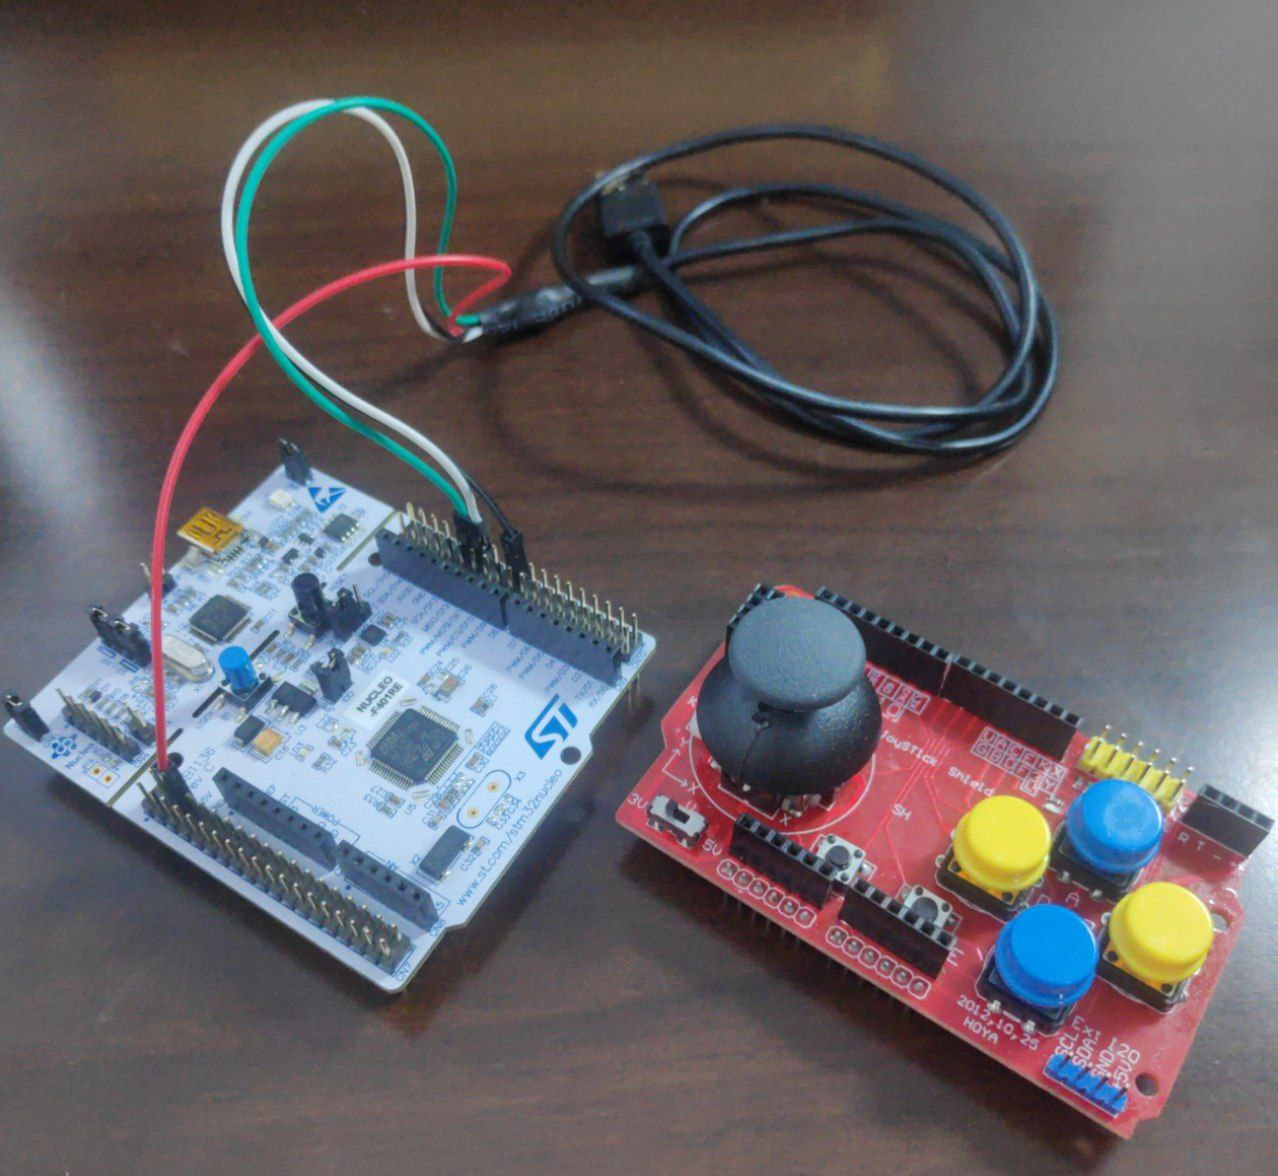
\includegraphics[width=\linewidth]{setup.jpg}
  \caption{Configuração de exemplo.}
  \label{fig:setup}
\end{figure}

\clearpage
\pagestyle{body}

\section{Visão Geral}
Human Interface Devices (HID), ou Dispositivos de Interface Humana, são equipamentos que interagem traduzindo estímulos de entrada e saída de/para seres humanos em estímulos para/de computadores. Exemplos comuns de HIDs são teclados, mouses, telas, botões e joysticks. Para promover um protocolo generalizado destes dispositivos e permitir que eles tenham a qualidade "Plug-and-Play" (i.e. diferentes componentes de hardware com uma mesma especificação podem ser conectados sem configuração por parte do usuário), há um padrão HID publicado pelo USB Implementers Forum.

\section{Descrição do Firmware}
A biblioteca de USB disponibilizada pela ST como Middleware no software STM32CubeMX provê alguns arquivos úteis para esta aplicação:

Middleware da biblioteca:
\begin{itemize}
    \item \texttt{usbd\_core.c} (cerne das funcionalidades)
    \item \texttt{usbd\_ioreq.c, usbd\_ctlreq.c} (requisições IO)
    \item \texttt{usbd\_hid.c} (trata das interações com o Host)
\end{itemize}

Arquivos de aplicação:
\begin{itemize}
    \item \texttt{usbd\_conf.c} (funções LL/HAL)
    \item \texttt{usbd\_device.c} (funções de inicialização)
\end{itemize}

Destes arquivos, vale destacar o \texttt{usbc\_hid.c}, que contém os descritores do dispositivo USB. Esses descritores servem para que o computador (Host) saiba com qual tipo de dispositivo está lidando (e.g. mouse, teclado, etc.) e como interpretar os pacotes (reports) que está recebendo. Por default, o STM32CubeMX gera descritores para um mouse e assim será usado nesta aplicação.

Obs.: A placa de desenvolvimento usada suporta somente USB FullSpeed (12 Mbits/s), apesar de haver Middleware disponível para USB HighSpeed (480 Mbit/s).

\subsection{Descritores}
Dos vários descritores gerados no arquivo \texttt{usbd\_hid.c}, dois são particularmente interessantes de serem analisados:

\paragraph{USBD\_HID\_CfgFSDesc} é o descritor de configurações de USB HID e contém uma série de informações gerais sobre o dispositivo, como corrente de alimentação, número de interfaces, código do país, entre muitas outras.

\paragraph{HID\_MOUSE\_ReportDesc} é um descritor dos \texttt{reports}, que são os pacotes de dados enviados pelo Device para o Host. A função deste descritor é informar ao Host como ele deve esperar que os dados do \texttt{report} cheguem, e como entendê-los assim que eles são recebidos. Aqui é que fica definido que o dispositivo é um mouse - ou teclado, ou o que seja -, quais são os valores máximos e mínimos dos campos de entrada, tamanho do report, entre outras informações.

Para gerar estes descritores, pode-se ler as definições de protocolo USB, encontrá-los gerados para uma aplicação semelhante e alterá-los, ou usar o gerador oficial chamado \textbf{HID Descriptor Tool}.

Segue abaixo, a interpretação dos valores do descritor \texttt{HID\_MOUSE\_ReportDesc}:

\begin{minted}
[
frame=lines,
framesep=2mm,
baselinestretch=1.2,
bgcolor=LightGray,
fontsize=\footnotesize,
]
{C}
0x05, 0x01, // Usage Page (Generic Desktop Ctrls)
0x09, 0x02, // Usage (Mouse)
0xA1, 0x01, // Collection (Application)
0x09, 0x01, // Usage (Pointer)
0xA1, 0x00, // Collection (Physical)
0x05, 0x09, // Usage Page (Button)
0x19, 0x01, // Usage Minimum (0x01)
0x29, 0x03, // Usage Maximum (0x03)
0x15, 0x00, // Logical Minimum (0)
0x25, 0x01, // Logical Maximum (1)
0x95, 0x03, // Report Count (3)
0x75, 0x01, // Report Size (1)
0x81, 0x02, // Input
0x95, 0x01, // Report Count (1)
0x75, 0x05, // Report Size (5)
0x81, 0x01, // Input
0x05, 0x01, // Usage Page (Generic Desktop Ctrls)
0x09, 0x30, // Usage (X)
0x09, 0x31, // Usage (Y)
0x09, 0x38, // Usage (Wheel)
0x15, 0x81, // Logical Minimum (-127)
0x25, 0x7F, // Logical Maximum (127)
0x75, 0x08, // Report Size (8)
0x95, 0x03, // Report Count (3)
0x81, 0x06, // Input
0xC0,       // End Collection
0x09, 0x3C, // Usage (Motion Wakeup)
0x05, 0xFF, // Usage Page (Reserved 0xFF)
0x09, 0x01, // Usage (0x01)
0x15, 0x00, // Logical Minimum (0)
0x25, 0x01, // Logical Maximum (1)
0x75, 0x01, // Report Size (1)
0x95, 0x02, // Report Count (2)
0xB1, 0x22, // Feature
0x75, 0x06, // Report Size (6)
0x95, 0x01, // Report Count (1)
0xB1, 0x01, // Feature
0xC0,       // End Collection
\end{minted}

\subsection{Configuração}
% O que tem de ser colocado na main.c para o HID funcionar.

As modificações necessárias para o uso do HID são poucas e podem ser divididas em 3 grupos, include, criação do handle e envio dos comandos, todos os três grupos serão explicados a seguir.

\subsubsection{Biblioteca}

O código da main precisa incluir somente a biblioteca principal do HID. Ela deve ser modificada para selecionar o tipo de dispositivo que será apresentado ao computador, nos termos indicados pelo parágrafo sobre HID\_MOUSE\_ReportDesc.

\begin{minted}
[
frame=lines,
framesep=2mm,
baselinestretch=1.2,
bgcolor=LightGray,
fontsize=\footnotesize,
]
{C}
#include "usbd_hid.h"
\end{minted}

\subsubsection{Handle necessário}

Para o uso do HID é requerido um handle que manipule os dados necessários para a comunicação USB e é declarado desta forma:

\begin{minted}
[
frame=lines,
framesep=2mm,
baselinestretch=1.2,
bgcolor=LightGray,
fontsize=\footnotesize,
]
{C}
USBD_HandleTypeDef hUsbDeviceFS;
\end{minted}

\subsubsection{Envio de dados}
O código desta etapa deve ser utilizado todas as vezes que for enviar dados para o computador.
Os dados precisam ser passados para a função em um bloco de bytes, em nosso exemplo utilizamos a estrutura abaixo para o envio de dados de um mouse. Nessas condições o payload tem 4 bytes e é organizado da seguinte forma:

\begin{minted}
[
frame=lines,
framesep=2mm,
baselinestretch=1.2,
bgcolor=LightGray,
tabsize=4,
fontsize=\footnotesize,
]
{C}
struct mouseHID_t {
	uint8_t buttons;
	int8_t x;
	int8_t y;
	int8_t wheel;
};
\end{minted}

A única coisa que nos resta é enviar os dados armazenados por meio da função. Como a função foi implementada esperando como entrada um ponteiro para int8\_t, fazemos um cast e então chamamos a função.

\begin{minted}
[
frame=lines,
framesep=2mm,
baselinestretch=1.2,
bgcolor=LightGray,
tabsize=4,
fontsize=\footnotesize,
]
{C}
uint8_t * buff = (uint8_t *) &mouseHID;
USBD_HID_SendReport(&hUsbDeviceFS, buff,
                    sizeof(struct mouseHID_t));
\end{minted}


\section{Descrição do Hardware}

O STM32F401 possui periférico específico para comunicação via USB e para o seu funcionamento somente é necessário interligar um conector USB aos pinos disponibilizados pelo hardware para esta função.

\paragraph{A placa} utilizada é a Nucleo-F401RE, para a utilização como HID ela precisa ser alimentada pela mesma conexão que será utilizada e este processo deve ser feito  colocando o jumper PWR na posição E5V. Lembrando que para o processo de gravação é necessário que o jumper esteja na posição U5V.

\paragraph{O cabo} utilizado é um cabo USB simples com conector dupont fêmea.

\paragraph{O shield}apesar do shield não ser necessário para a utilização do HID ele é essencial para o exemplo disponibilizado junto a essa Application note. Ele se chama Joystick Shield V1.A
estão descritas na tabela a seguir e devem ser utilizadas na função pull-up.

\subsection{Setup de hardware}

Para utilizar o HID é necessário simplesmente conectar os fios do cabo USB na placa seguindo a tabela a seguir e encaixar o Joystick Shield V1.A nos conectores compatíveis com o Arduino.

\vspace*{10pt}
\fboxsep=2mm \fboxrule=0.2mm

\begin{table}[ht]
\centering
\begin{tabular}{|l l c|}
\hline
USB & MCU & Cor do fio\\
\hline
+5V & E5V & \fcolorbox{black}{red}{\null}\\
D- &  PA11 & \fcolorbox{black}{white}{\null}\\
D+ & PA12 & \fcolorbox{black}{green}{\null}\\
GND & GND & \fcolorbox{black}{black}{\null}\\
\hline
\end{tabular}
\caption{Conexões do USB.}
\label{tab:usb}
\end{table}

O shield tem todas as conexões utilizadas fixas, mas vale a pena evidenciá-las para a melhor compreensão do funcionamento do código. As conexões estão dispostas na tabela \ref{tab:shield}:


\begin{table}[H]
\centering
\begin{tabular}{|c l|}
\hline
Função & MCU\\
\hline
A & PA10\\
B & PB3\\
C & PB5\\
D & PB5\\
E & PB10\\
F & PA8\\
K & PA9\\
X & PA0\\
Y & PA1\\
\hline
\end{tabular}
\caption{Conexões do shield.}
\label{tab:shield}
\end{table}

\section{Reproduzindo o Exemplo}


O exemplo foi projetado para a utilização do Joystick Shield V1.A como HID reproduzindo o comportamento de um mouse. O joystick, propriamente dito, controla o movimento do mouse, os botões A e C executam a rolagem para cima e para baixo, os botões D, F e K o clique primário e os botões B e E o clique secundário. 

\subsection{STM32CubeMX}
Para reproduzir o exemplo, crie um projeto em branco para a placa STM32F401RE Nucleo64 no STM32CubeMX. Quando perguntado se deseja inicializar os periférico no modo deafult, selecione "Não".

\paragraph{Encontre} na aba \textbf{"Pinout \& Configuration"} a configuração\\ \textit{System Core $\rightarrow$ RCC $\rightarrow$ High Speed Clock (HSE)}\\ e selecione a opção \textbf{BYPASS Clock Source} como na imagem \ref{fig:ex0}.

\begin{figure}[H]
  \centering
  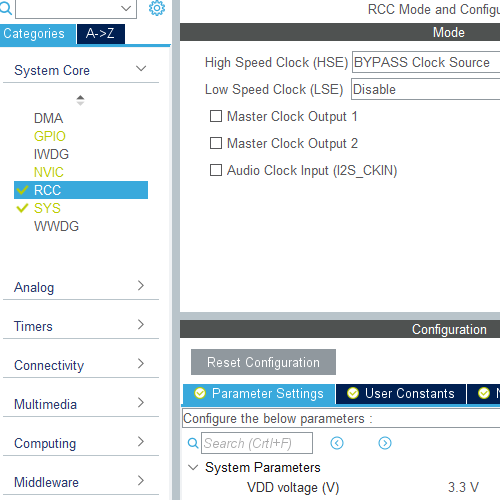
\includegraphics[width=0.8\linewidth]{0_cube_RCC_HSE.png}
  \caption{Configurar RCC para BYPASS Clock Source.}
  \label{fig:ex0}
\end{figure}

\paragraph{Depois disso,} configure os pinos descritos na tabela \ref{tab:shield} como GPIO no modo input com pull-up ativado.

\paragraph{Em seguida,} ative as configurações\\ \textit{Analog $\rightarrow$ ADC1 $\rightarrow$ IN0 e IN1}\\como na figura \ref{fig:ex1}.

\begin{figure}[H]
  \centering
  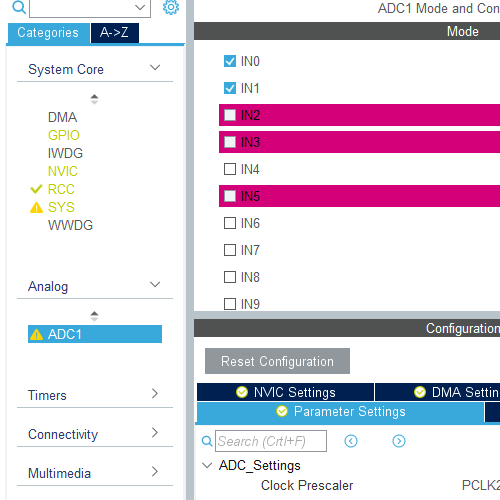
\includegraphics[width=0.8\linewidth]{1_cube_adc.png}
  \caption{Ativar ADC para as portas IN0 e IN1.}
  \label{fig:ex1}
\end{figure}

\paragraph{Configure} o USB em \\ \textit{Connectivity $\rightarrow$ USB\_OTG\_FS $\rightarrow$ Mode}\\ para \textbf{Device only}, como na figura \ref{fig:ex2}.

\begin{figure}[H]
  \centering
  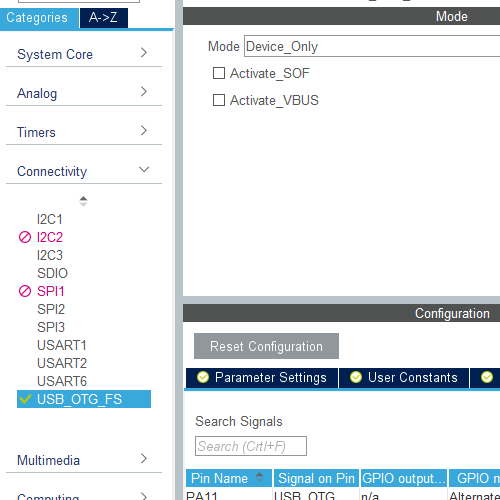
\includegraphics[width=0.8\linewidth]{2_cube_USB_Device.png}
  \caption{Configurar USB para o modo Device Only.}
  \label{fig:ex2}
\end{figure}

\paragraph{Na configuração}:\\ \textit{Middleware $\rightarrow$ USB\_DEVICE $\rightarrow$ Class For FS IP}\\ Selecione a opção \textbf{Human Interface Device Class (HID)}, como na figura \ref{fig:ex3}.

\begin{figure}[H]
  \centering
  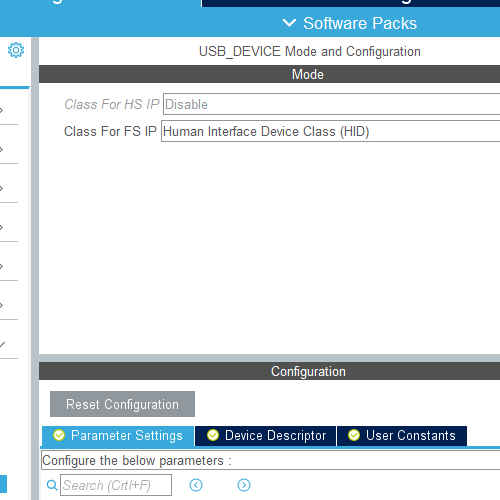
\includegraphics[width=0.8\linewidth]{3_cube_USB_ClassFS.png}
  \caption{Configurar USB para o modo HID.}
  \label{fig:ex3}
\end{figure}

\paragraph{Na aba} \textbf{Clock Configuration} aparecerá a mensagem de erro abaixo (figura \ref{fig:ex3}). Selecione "Yes" e após alguns instantes a árvore de clock deve parecer com a figura \ref{fig:ex4}.

\begin{figure}[h]
  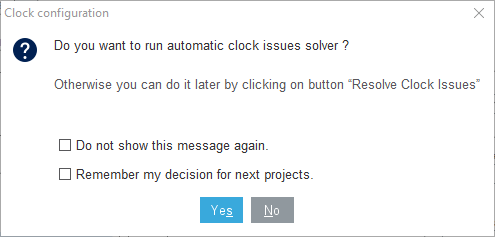
\includegraphics[width=0.8\linewidth]{4_cube_clock_problem.png}
  \caption{Problema com o clock.}
  \label{fig:ex4}
\end{figure}

\paragraph{Por fim,} configure o nome e local do projeto e gere o código com a toolchain de preferência. Neste projeto foi usada a \textbf{SW4STM32}.

\subsection{SW4STM32}
A IDE usada neste projeto foi a \textbf{SW4STM32}. Para finalizar o projeto basta configurar os arquivos gerados pelo \textbf{STM32CubeMX} segundo a seção \textbf{Descrição do Firmware} deste documento e gravar na placa de desenvolvimento.

\subsection{Executando o Exemplo}
\paragraph{A gravação do exemplo}pode ser feita a partir da gravação direta do .elf disponibilizado ou também pela compilação própria do código acessível pelo repositório ou pelo arquivo gerado.

\paragraph{IMPORTANTE!} O jumper \textbf{JP5} (PWR) define a origem da alimentação da placa. Para gravar, o jumper deve estar na posição \textbf{U5V} (alimentação pelo STLink) e o USB-Dupont deve estar desconectado da energia. Após a gravação o jumper deve ser colocado na posição necessária para o HID, isto é, ligando o pino central ao \textbf{E5V} (alimentação externa pelo USB-Dupont) e o cabo do STLink deve ser desconectado da energia.

\newpage
\clearpage
\pagestyle{last}
\begin{onecolumn}
\begin{table}[!ht]%
\caption{Histórico de revisões.}
\label{}
\centering
\begin{tabular}{p{0.3\linewidth}p{0.3\linewidth}p{0.3\linewidth}}
\hline
Revisão & Autores & Modificações\\
\hline
0.1 & Luis Lindgren e João Falcão & Lançamento inicial da Application Note\\
\hline
\end{tabular}
\end{table}
\end{onecolumn}

\end{document}

